%L’expérience que nous avons réalisé consiste donc à réaliser des transistors moléculaires, afin de caractériser leur comportement.
\section{La réalisation des circuits en salle blanche (faite en amont par Mr Balestro)}
La réalisation des fils d’or a pris plusieurs semaines ; c’est pourquoi Frank Balestro les avait déjà réalisés en salle blanche, au CNRS, avant l’expérience.
Nous avons donc commencé la journée avec 3 plaques de Al$_2$O$_3$, avec chacune 4 groupes de 12 transistors non formés.
\begin{figure}[h]
    \begin{center}
        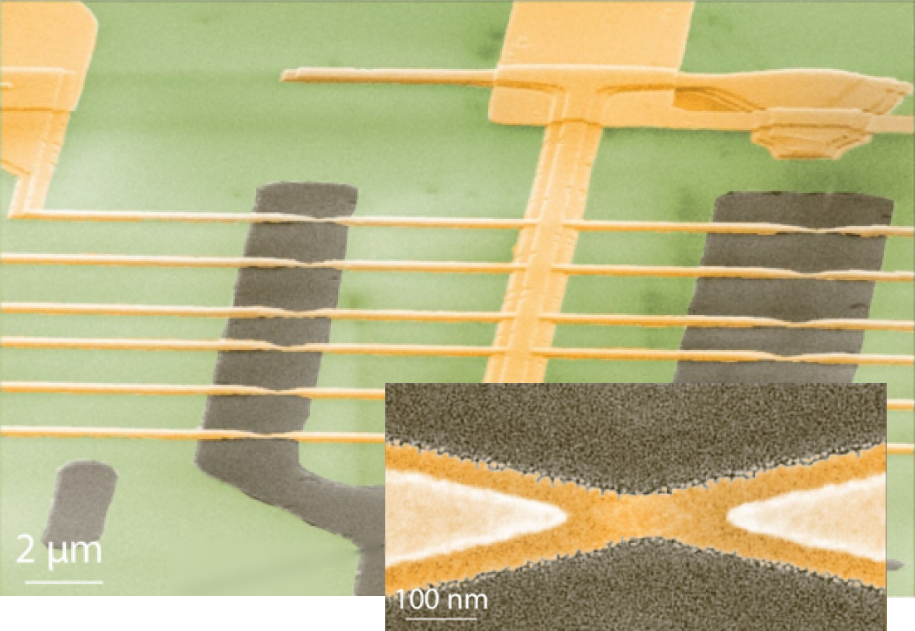
\includegraphics[width=250px]{Images/GroupeDeTransistors}
        \caption{Un groupe de transistors avec grille et source communes}
        \label{fig:}
    \end{center}
\end{figure}
\section{Le dépôt de Fullerène}
Nous sommes donc allés en salle blanche afin de déposer sur ces plaques le Fullerène, en solution de Toluène.
Cette solution, conservée dans un frigo, est parfaitement inerte, ce qui nous autorise à la conserver très longtemps : celle que nous avons utilisé date de 2009 et est encore utilisable.\\

Le dépôt se fait à l’aide d’une micropipette, et sous hotte aspirante afin d’éviter toute inhalation de fullerène.
La solution est assez faible en agrégats, et ceux qui ont pu se former se trouvent essentiellement à la surface et au fond de la solution. Nous sommes donc allés récupérer la solution au milieu du bécher.

Le dépôt de fullerène n’a pas besoin d’être quantitativement : 3 gouttes de solution par plaque sont suffisantes pour obtenir une probabilité acceptable qu’une molécule se glisse dans le nanogap après électromigration.

Enfin, nous avons laissé s’évaporer le Toluène.
\section{Une expérience à 4.2K grâce à l'hélium liquide}
\begin{figure}[h]
    \begin{center}
        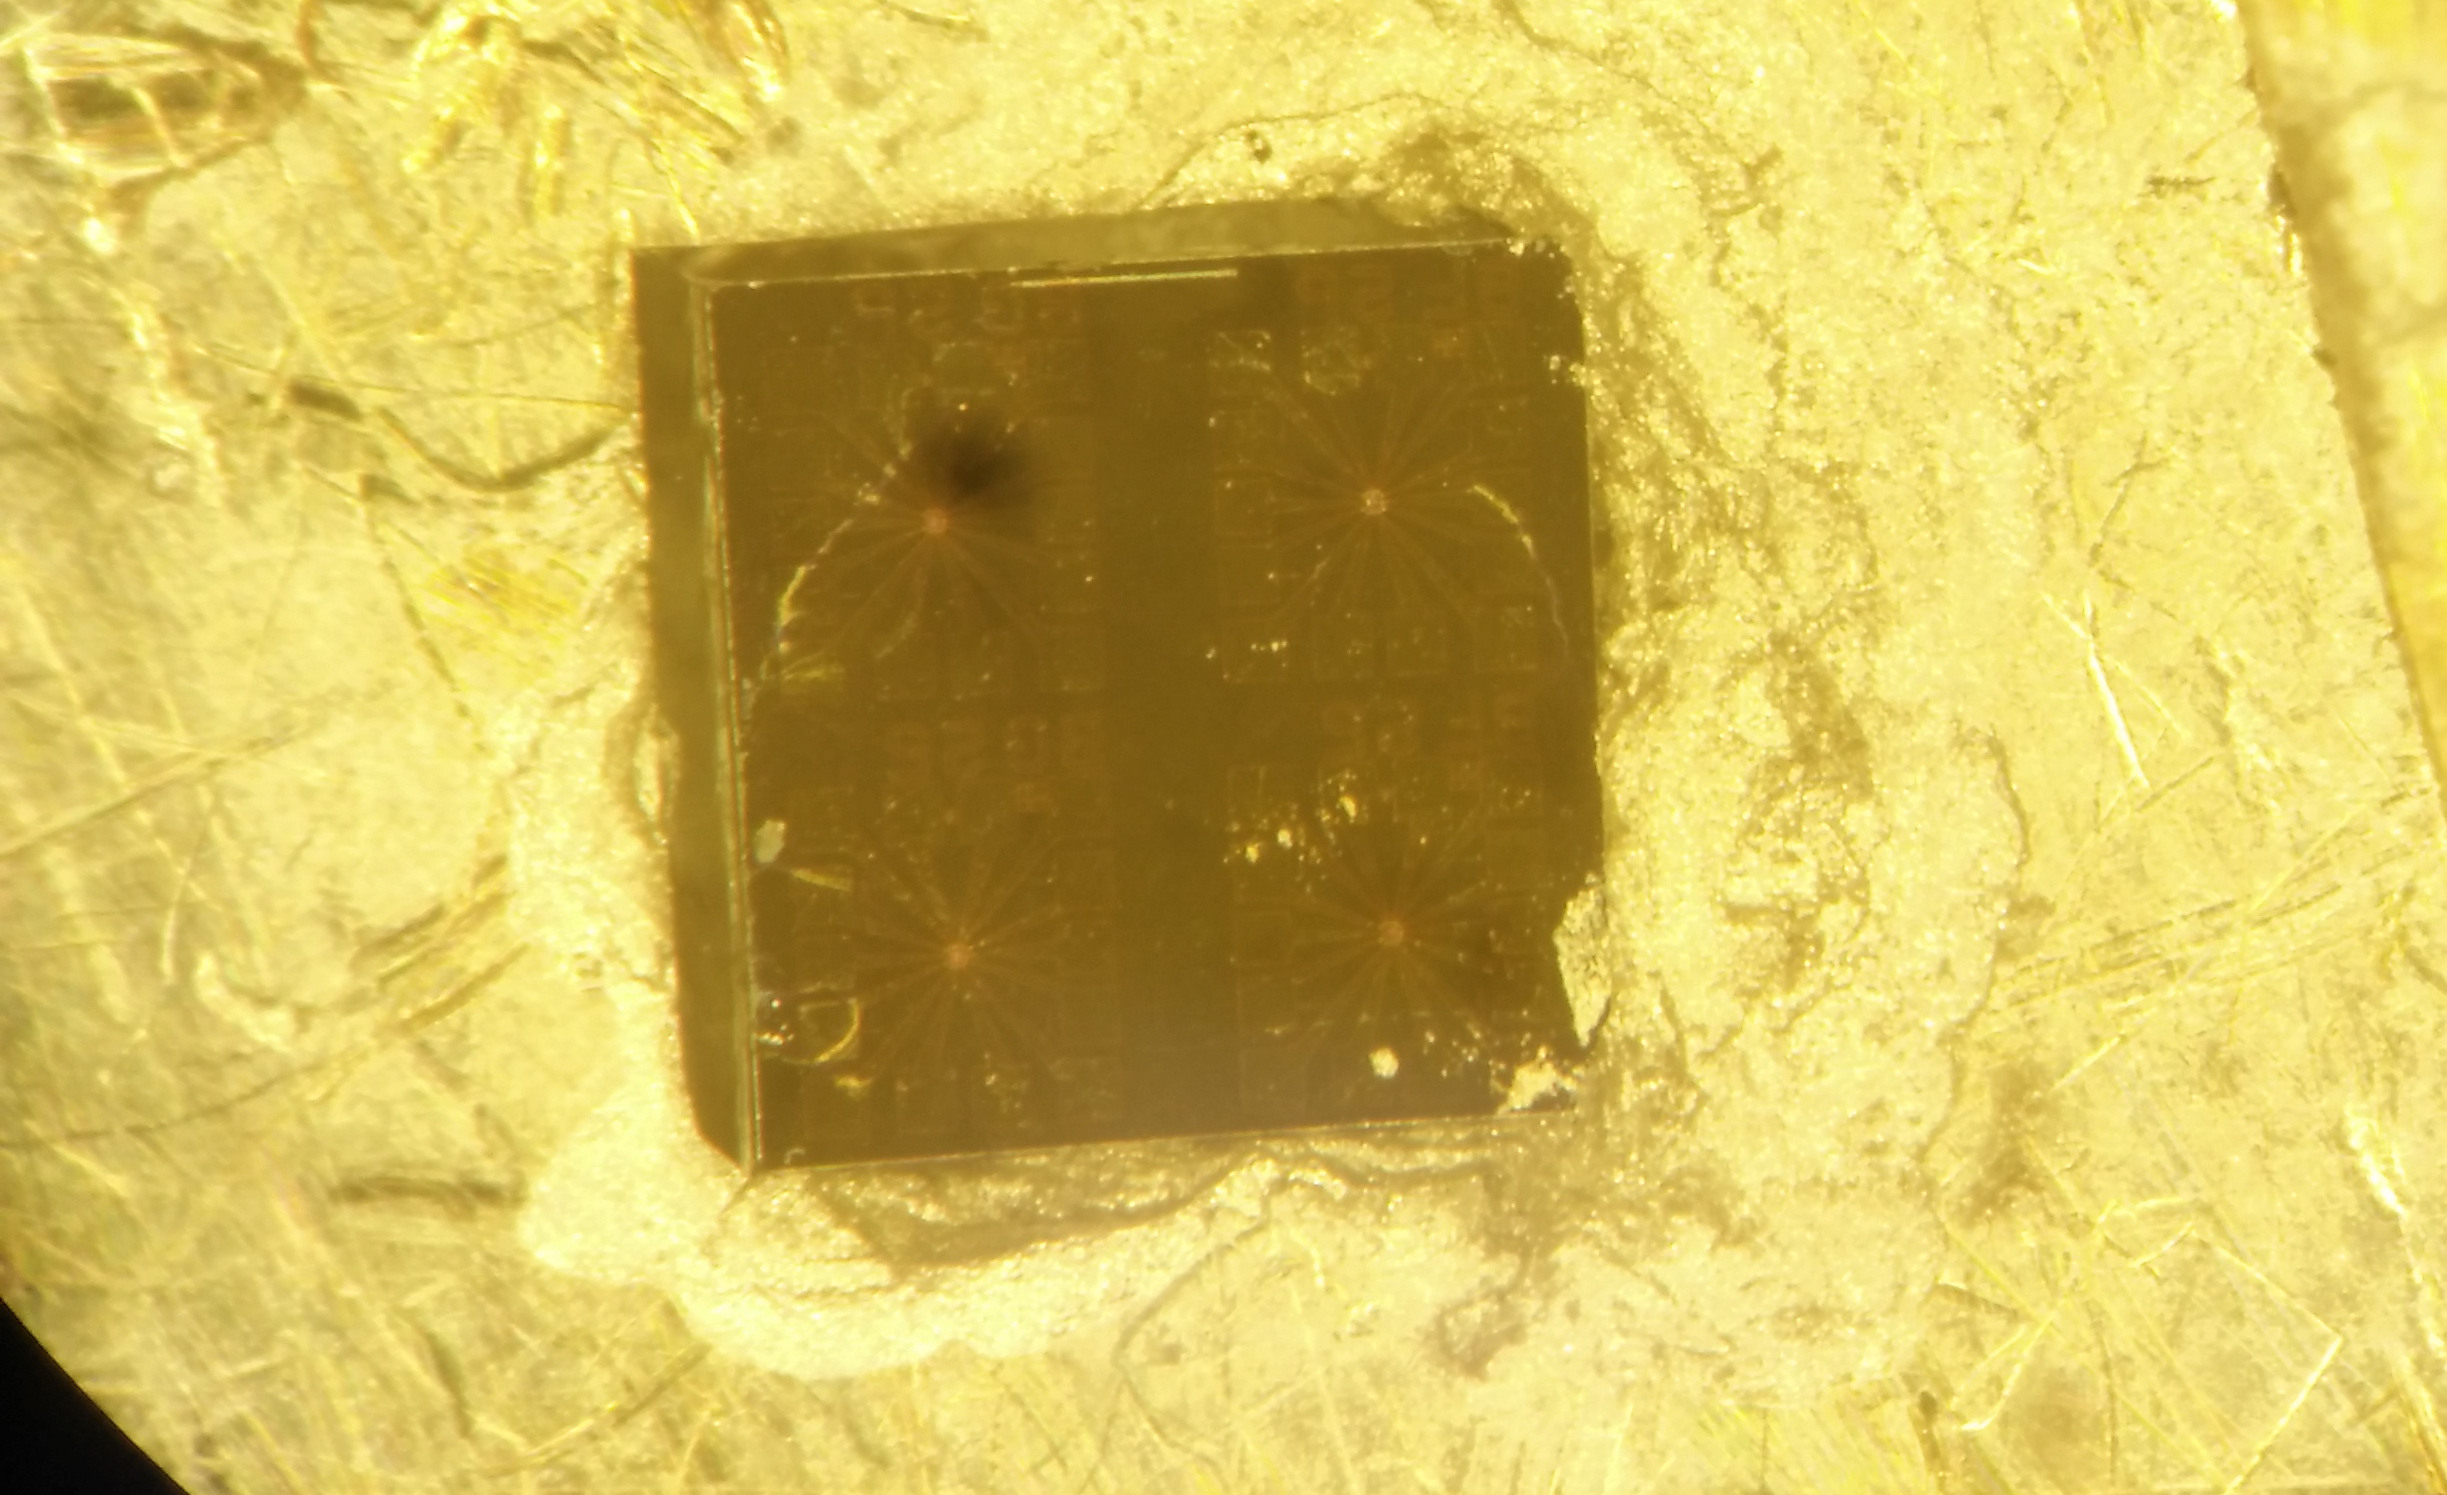
\includegraphics[width=250px]{Images/PhotoPlaqueTransistors}
        \caption{Une plaque "collée" sur le plateau métallique}
        \label{fig:}
    \end{center}
\end{figure}
\section{Comment effectuer les mesures}
